\chapter{Vorstellung von Apache Spark}
Aus Sicht eines Nutzers ist Apache Spark eine API zum Zugriff auf Daten und deren Verarbeitung.\\

Diese API (wahlweise für die Programmiersprachen Scala, Java und Python verfügbar), kann im einfachsten Fall über eine eigene Spark Konsole mit \gls{repl}\cite{Hail} verwendet werden.\\
Die Zählung von Wortvorkommen in einem Text - das "`Hello World"' der Big Data Szene - lässt sich dort mit zwei Befehlen realisieren (Listing \ref{lst:sconsole_wordcount}).\\

\begin{lstlisting}[language=Scala,caption={Word Count in der Spark Konsole},label={lst:sconsole_wordcount}]
my_dollar ./spark-shell
[...]
     / __/__  ___ _____/ /__
    _\ \/ _ \/ _ `/ __/  '_/
   /___/ .__/\_,_/_/ /_/\_\   version 1.3.0
      /_/
Using Scala version 2.10.4 (OpenJDK 64-Bit Server VM, Java 1.7.0_75)
Type in expressions to have them evaluated.
[...]
scala> val text = sc.textFile("../Heinrich Heine - Der Ex-Lebendige")
[...]
scala> :paste
text.flatMap(line => line.split(" "))
.map(word => (word, 1))
.reduceByKey(_ + _)
.collect()
[...]
res0: Array[(String, Int)] = Array((Tyrann,,1), (im,2), (Doch,1) ...)
\end{lstlisting}


Aus Sicht eines Administrators oder Softwarearchitekten ist Apache Spark eine Applikation auf einem \gls{cluster}, die sich in der Anwendungsschicht befindet und charakteristische Anforderungen insbesondere an Lokalität des Storages und die Netzwerkperformance stellt.\\

Was das konkret bedeutet, welche Mechanismen und Konzepte dahinterstehen und in welchem Ökosystem von Anwendungen sich Apache Spark bewegt wird in den folgenden Abschnitten dieses Kapitels beleuchtet.

\section{Überblick}
Im Allgemeinen Fall läuft eine Spark-Anwendung auf drei Arten von Rechnern (s. Abb.~\ref{fig:sparkdeployment}):

\begin{enumerate}
	\item \textbf{Clientknoten}\\
	Auf Nutzerseite greift die Anwendung auf die API eines lokalen Spark-Kontextes zu, der die Kontaktdaten eines Clustermanagers sowie verschiedene Konfigurationseinstellungen enthält. 
	
	\item \textbf{\gls{master}knoten}\\
	Der \gls{master}knoten betreibt den \textit{Clustermanager}, läuft auf einem entfernten Rechner und ist der Einstiegspunkt in den \gls{cluster}. Hier werden Aufträge des Anwenders an die Arbeitsknoten verteilt und Ergebnisse eingesammelt und zurückgereicht.
	
	\item \textbf{\gls{worker}knoten}\\
	Die \gls{worker}knoten beherbergen die Spark \textit{Executors} und sind die ausführenden Elemente der Aktionen und Transformationen. Die \textit{Executors} können untereinander Zwischenergebnisse austauschen und melden ihre Ressourcenverfügbarkeit an den \textit{Clustermanager}.
\end{enumerate}

\begin{figure}[ht!]
	\centering
  \includegraphics[scale=0.7]{sparkdeployment2.pdf}
	\caption{Verteilungsdiagramm einer typischen Sparkinstallation}
	\label{fig:sparkdeployment}
\end{figure}

Um die Architektur und Optimierungskonzepte eines verteilten Systems bewerten zu können ist es offensichtlich wichtig, welche Eigenschaften der unterliegenden Hardware angenommen werden.

Weil Spark explizit für den Betrieb innerhalb eines Hadoop/YARN \textcolor{red}{[VERWEIS auf Abschnitt Scheduling]} geeignet ist und YARN wiederum für den Betrieb auf einem \gls{cluster} auf Mittelklasse-Mehrzweckmaschinen (Commodity Hardware) optimiert ist\cite{Mer14}, kann für Spark von einer vergleichbaren Hardwarekonfiguration ausgegangen werden.\\

Der Vergleich von drei aktuellen Rack Servern der 2000-Euro-Klasse (in der Grundausstattung) - hier als Mittelklasse-Geräte bezeichnet - liefert die folgenden Verhältnisse der wesentlichen Schnittstellen zueinander (Siehe Anhang~\ref{subsec:commodity_servers}).

\begin{table}[ht]
	\centering % used for centering table
	\begin{tabular}{c c c} % centered columns (4 columns)	
		\hline\hline %inserts double horizontal lines
		Netzwerk & Festspeicher & Arbeitsspeicher\\ [0.5ex] % inserts table
		%heading
		\hline % inserts single horizontal line
		0,125 GB/s & 1 GB/s & 17 GB/s \\ % inserting body of the table
		\hline %inserts single line
	\end{tabular}
	\caption{Theoretische Spitzenleistungen bei Mittelklasse-Servern} % title of Table
	\label{table:vgldurchsatz} % is used to refer this table in the text
\end{table}

Eine detaillierte Analyse des Zugriffsverhaltens ist nicht Gegenstand dieser Arbeit. Bei den folgenden Bewertungen der Kernkonzepte ist es wichtig sich die aus Tabelle \ref{table:vgldurchsatz} abgeleiteten Größenordnungen des Durchsatzes (\textit{D}) der verschiedenen Datenkanäle zu vergegenwärtigen:

\begin{equation*}
	D_{Netzwerk} < D_{Festspeicher} < D_{Arbeitsspeicher}
\end{equation*}

Für eine effiziente Verarbeitung von Daten ist es - ganz allgemein - also wünschenswert den größten Anteil des Datentransfers im Arbeitsspeicher zu haben, einen kleineren Anteil auf der Festplatte und einen noch kleineren Anteil auf Netzwerkverbindungen.\\

Es ist das wichtigste Ziel der folgenden Kernkonzepte von Apache Spark unter diesen Bedingungen die effiziente und stabile Verarbeitung \textit{großer Datenmengen}\cite{Sam14} zu gewährleisten.\\

\section{Kernkonzepte}

\subsection{Resilient Distributed Datasets}
Die universelle Einheit mit der Datenelemente auf Spark repräsentiert wird ist ein sogenanntes \gls{rdd}\cite{Mat12}.\\

Ein Beispiel für ein solches \gls{rdd} wurde bereits erwähnt, nämlich das in Listing \ref{lst:sconsole_wordcount} erzeugte Objekt \lstinline|text|:\\

\begin{lstlisting}[language=Scala]
val text = sc.textFile("../Heinrich Heine - Der Ex-Lebendige")
\end{lstlisting}

\Glspl{rdd} können auch explizit von einem Treiberprogramm erzeugt werden, ohne dass dazu vorhandene Daten genutzt werden:\\

\begin{lstlisting}
val listRDD = sc.parallelize(List(1,2,3,4,5,6))
\end{lstlisting}

Die gesamte operative Kern-\gls{api} dreht sich um die Steuerung dieser Dateneinheiten. Insbesondere sind auch die in den Standardbibliotheken verfügbaren "`höheren"' \glspl{api} auf diesen \glspl{rdd} implementiert.

Sie sind damit die wichtigste Abstraktion des Applikationskerns.\\

In erster Näherung können \glspl{rdd} als eine Variante von \gls{dsm}\cite{Nitzberg:1991:DSM:112827.112855} \cite{Mat12} verstanden werden, haben allerdings sehr charakteristische Einschränkungen und Erweiterungen, die in diesem Kapitel erläutert werden.\\

\paragraph{Verteilungssicht}\\

Aus Verteilungssicht ist ein \gls{rdd} ein Datensatz, der über den Arbeitsspeicher mehrerer Maschinen partitioniert ist (Abb.~\ref{fig:rdds1}).

\begin{figure}[ht!]
	\centering
  \includegraphics[scale=0.7]{RDDs1.pdf}
	\caption{Resilient Distributed Datasets aus Verteilungssicht}
	\label{fig:rdds1}
\end{figure}

\paragraph{Laufzeitsicht}\\

\Glspl{rdd} sind nicht veränderbar. Es ist nicht möglich einzelne Elemente \gls{RDD} durch gezielte Operationen zu verändern. Stattdessen ist es nur möglich ein einmal definiertes \gls{rdd} durch globale Anwendung von Operationen in ein anderes zu überführen.\\
Solche globalen (also auf sämtlichen Partitionen des \gls{RDD} durchgeführten) Operationen können zwar ihren Effekt auf einzelne Elemente eines \gls{RDD} beschränken, die Ausführung erfolgt jedoch in jedem Fall auf allen Partitionen.\\

Eine Folge von Operationen $op_1op_2op_3...$ wird als \textit{Lineage} eines \gls{rdd} bezeichnet. Die \textit{Lineage} kann als das "`Rezept"' zur Erstellung eines Datensatzes verstanden werden.

Dabei gibt es zwei grundsätzlich verschiedene Operationen, nämlich \textit{Transformationen} und \textit{Aktionen}.\\

\textbf{\textit{Transformationen}} sind Operationen, die ein \gls{RDD} auf ein anderes Abbilden:\\
\[Transformation: RDD \times RDD\ \longrightarrow RDD\]
oder
\[Transformation: RDD\ \longrightarrow RDD\]
\\
Es werden also - grob gesagt - nur die abstrakte Repräsentation des Datensatzes ändern, ohne tatsächlich dessen Datenelemente für den Programmfluss im Treiberprogramm abzurufen.\\
Beispiele für solche Operationen sind:
\begin{itemize}
	\item \textit{filter}
	\item \textit{join}
\end{itemize}\\

\textbf{\textit{Aktionen}} sind Operationen, die \glspl{rdd} in eine andere Domäne abbilden:\\
\[Action: RDD \longrightarrow Domain_x, Domain_x \neq RDD\]
\\
Beispiele für Aktionen sind die Methoden:
\begin{itemize}
	\item \textit{reduce}
	\item \textit{count}
	\item \textit{collect}
	\item \textit{foreach}
\end{itemize}\\

Jeder dieser Operationen, kann im Sinne des Command-Patterns (\cite{FPP13}) eine Funktion bzw. ein Funktionsobjekt übergeben werden, dass die gewählte Operation spezifiziert.

Solange nur \textit{Transformationen} auf einem \gls{rdd} ausgeführt werden, ist dieses noch ein bloßes "`Rezept"' zur Erstellung eines Datensatzes. Tatsächlich wurde noch kein Speicher reserviert und der Cluster wurde noch nicht aktiv\cite{Mat12}:\\

\begin{figure}[ht!]
	\centering
  \includegraphics[scale=0.8]{rdds_no_action.pdf}
	\caption{RDD Lineage vor Aktion (gestrichelte Linie steht für \textit{nicht initialisiert}}
	\label{fig:rdds_no_action}
\end{figure}

Sobald die erste \textit{Aktion} aufgerufen wird, werden die Transformationen nach der vorgegebenen Reihenfolge ausgeführt und die geforderte \textit{Aktion} ausgeführt. Die Initialisierung des \gls{rdd} erfolgt also "`lazy"':\\

\begin{figure}[ht!]
	\centering
  \includegraphics[scale=0.8]{rdds_action.pdf}
	\caption{RDD Lineage nach Aktion}
	\label{fig:rdds_action}
\end{figure}

Wie in Abb. \ref{fig:rdds_action} dargestellt ist, werden während der Transformationsvorgänge keine Zwischenergebnisse gespeichert. Möchte man Zwischenergebnisse zu einem späteren Zeitpunkt oder in anderem Zusammenhang wiederverwenden, kann man dies explizit über das Kommando \lstinline|persist()| anweisen:\\

\begin{figure}[ht!]
	\centering
  \includegraphics[scale=0.8]{rdds_action_persist.pdf}
	\caption{RDD Lineage nach Aktion und mit Persist()}
	\label{fig:rdds_action_persist}
\end{figure}
\\
Realisiert ist das Konzept der \textit{Lineage} und der "`Lazy Computation"' von \glspl{rdd} durch Transformations-Methoden, die eine Variante des Factory-Pattern (\cite{FPP13}) implementieren. Die erzeugten Objekte sind dabei wiederum Unterklassen von \gls{rdd}:\\
Jedes \gls{rdd}-Objekt führt eine Liste von Vorgängern mit. Aus dieser lässt sich auch die Art der Berechnung des jeweiligen Nachfolgers ableiten.\\

Jede weitere Transformations-Methode konstruiert nun lediglich eine neues \gls{rdd}-Objekt. Dieses basiert auf dem aktuellen Objekt und der jeweiligen Transformation.\\

Ein Beispiel für solch eine Transformation auf einem \gls{rdd} ist die Methode \textit{map}\footnote{https://github.com/apache/spark/blob/branch-1.3/core/src/main/scala/org/apache/spark/rdd/RDD.scala#L285 (abgerufen am 30.05.2015)} (Listing \ref{lst:spark_map}).\\

In den Zeilen 7 und 8 ist zu sehen, wie ein neues \gls{rdd} erzeugt wird und diesem das aktuelle \gls{rdd} sowie die auf dessen Elemente anzuwendende Funktion \lstinline|f| (bzw. \lstinline|cleanF|) übergeben wird.\\

\begin{lstlisting}[language=Scala,caption={Map-Methode aus org.apache.spark.rdd.RDD v1.3.0},label={lst:spark_map}]
  /**
   * Return a new RDD by applying a function to all elements of 
	 * this RDD.
   */
  def map[U: ClassTag](f: T => U): RDD[U] = {
    val cleanF = sc.clean(f)
    new MapPartitionsRDD[U, T](this, (context, pid, iter) 
		  => iter.map(cleanF))
  }
\end{lstlisting}
\\
Die tatsächliche Berechnung eines \glspl{rdd} wird dann bei Aufruf einer Aktion gestartet. Als Beispiel hierfür sei die Methode \lstinline|foreach|\footnote{https://github.com/apache/spark/blob/branch-1.3/core/src/main/scala/org/apache/spark/rdd/RDD.scala#L793 (abgerufen am 30.05.2015)} aufgeführt (Listing \ref{lst:spark_foreach}).\\
In Zeile 6 wird auf dem Spark-Context die Methode \lstinline|runJob| aufgerufen, der die Aufgabe weiter an den Scheduler delegiert. Dort werden dann die rekursiven Abhängigkeiten des aktuellen \gls{rdd} aufgelöst und - je nach Konfiguration - die Tasks verteilt.\\

\begin{lstlisting}[language=Scala,caption={foreach-Methode aus org.apache.spark.rdd.RDD v1.3.0},label={lst:spark_foreach}]
  /**
   * Applies a function f to all elements of this RDD.
   */
  def foreach(f: T => Unit) {
    val cleanF = sc.clean(f)
    sc.runJob(this, (iter: Iterator[T]) => iter.foreach(cleanF))
  }
\end{lstlisting}
\\
Das Konzept der \textit{Lineage} ist zentral für die Fehlertoleranz der \gls{rdd}s:
Geht eine Partition verloren - beispielsweise durch Defekt eines Knotens - ist das "`Rezept"' zur Erstellung des Datensatzes in der \textit{Lineage} des \gls{rdd}-Objektes weiterhin vorhanden und die Partition kann gezielt wiederhergestellt werden.\\

Ein weiterer Vorteil dieser Art von Arbeitsdatensatz wird ebenfalls sofort deutlich: Im optimalen Fall sind die zu ladenden Daten von jedem der \gls{worker} auf unabhängigen Kanälen erreichbar (z.B. auf dem lokalen Festspeicher) und gleichmäßig auf diesen Kanälen partitioniert.\\

\begin{figure}[h!]
	\centering
  \includegraphics[scale=0.7]{RDDs2.pdf}
	\caption{Resilient Distributed Datasets mit Datenquelle aus Verteilungssicht}
	\label{fig:rdds2}
\end{figure}

Im diesem Fall ergäbe sich mit einer Anzahl \gls{worker} $n$ und einem Durchsatz $\delta$ zu der jeweiligen Datenquelle also ein idealer Gesamtdurchsatz beim Einlesen von Daten von:

\begin{equation}
	\sum_{i=1}^{n} \delta_i
\end{equation}

Kommen in einem Anwendungsfall \gls{rdd}s zum Einsatz, deren Elemente einzeln über eine oder mehrere Operationen untereinander verknüpft werden, kann es sinnvoll sein diese schon im Vorfeld der Verarbeitung entsprechend erwarteter Cluster zu partitionieren. Cluster seien hierbei Teilmengen des \gls{rdd}, die mit besonders hoher Wahrscheinlichkeit oder besonders häufig untereinander verknüpft werden.\\

Dadurch kann ein größerer Teil der Operationen auf den einzelnen Datensätzen bereits lokal auf dem Knoten der jeweiligen Partition durchgeführt werden. Die Netzwerklast bei dem anschließenden \textit{Shuffle} der Daten (siehe Abschnitt 2.2.2) fällt dann geringer aus.\\

Solch eine Partitionierung kann - entsprechende Erwartung über das Verhalten der Verarbeitung vorausgesetzt - mit einem maßgeschneiderten Partitionierer erreicht werden (Abb.~\ref{lst:partitioner}) der dann dem betroffenen \gls{rdd} übergeben wird.\\

\begin{lstlisting}[language=Scala,caption={Beispiel: Minimaler Partitionierer},label={lst:partitioner}]
/*
 * Beispiel für einen minimalen Partitionierer. 
 * Ueber selbstdefinierte Hash Codes kann hier eine 
 * massgeschneiderte physische Verteilung ueber die 
 * Knoten erreicht werden.
 */
class MinimalPartitioner extends Partitioner {
 def numPartitions = 10

 def getPartition(key: Any): Int =
   key.hashCode % numPartitions
	
 def equals(other: Any): Boolean =
   other.isInstanceOf[MinimalPartitioner]
}
\end{lstlisting}

\subsection{Scheduling/Shuffling}\\

Bisher wurden insbesondere drei Aspekte eines \gls{rdd} betrachtet:
\begin{itemize}
	\item die \textbf{Partitionierung} der Elemente über verschiedene Rechner
	\item die \textbf{Vorgänger} eines \gls{rdd} bezüglich dessen \textit{Lineage}
	\item die \textbf{Funktion} mit der ein \gls{rdd} aus einem oder mehreren direkten Vorgängern berechnet wird
\end{itemize}

Betrachtet man nur die Vorgänger-Beziehung, dann erhält man zunächst eine einfache Baumstruktur.\\

Betrachtet man zusätzlich die Partitionierung und die Funktion mit der \glspl{rdd} transformiert werden, sieht man einen wichtigen Unterschied zwischen verschiedenen Vorgängerbeziehungen:
\begin{itemize}
\item Solche deren einzelne Partitionen höchstens eine Vorgängerpartition haben
\item Solche bei denen mindestens eine Partition mehr als eine Vorgängerpartition hat
\end{itemize}

Wird eine Partition aus höchstens einer anderen erzeugt, lässt sich diese direkt auf dem selben Knoten berechnen. Werden jedoch verschiedene Partitionen benötigt um eine Folgepartition zu erzeugen stellt sich die Frage auf welchen Knoten das am Besten geschieht.\\
Spark unterteilt diese beiden Fälle in \textit{narrow dependencies} (erster Fall) und \textit{wide dependencies} (zweiter Fall) (\cite{Mat12}). 
Der Abhängigkeitsgraph eines \gls{rdd} wird nun in sogenannte \textit{Stages} zerlegt. Eine \textit{Stage} ist dabei ein Untergraph, dessen Elemente (von den Blättern in Richtung Wurzel betrachtet) auf eine gemeinsame \textit{wide dependency} stoßen.\\

Elemente innerhalb einer Stage, können nach dieser Konstruktion völlig unabhängig auf den Knoten berechnet werden, die die jeweilige Partition vorhalten. Pro Datenelement x kann in einer Art Pipeline die Transformation über die Elemente der Vorgänger-\glspl{rdd} lokal der Wert berechnet werden.\\

Für den Übergang zwischen Stages ist die Berechnung der Nachfolger etwas aufwändiger:\\

Um eine neue Partition aus mehreren Vorgänger-Partitionen zu erzeugen werden zunächst geeignete Ausführungsorte\footnote{Geeignete Ausführungsorte (\textit{preferred locations}) können sich z.B. aus dem Ort eines Blocks bei HDFS ermitteln lassen (Node-Local, Rack-Local, etc.) oder daraus, ob ein Executor bereits einen Datensatz geladen hat (Process-Local)} ermittelt, von denen dann jeder per geeignetem Partitionierer mindestens einen \textit{bucket} von Elementen verarbeitet. Diese Elemente stammen dann in der Regel aus verschiedenen Vorgängerpartitionen.\\
Das so neu-partitionierte und verarbeitete \gls{RDD} wird so zum Ausgangspunkt des folgenden \gls{rdd}.\\
Eine Schlüsselrolle kommt bei diesem Prozess der Methode \lstinline|runTask| in der Klasse 
\lstinline|ShuffleMapTasks|\footnote{https://github.com/apache/spark/blob/branch-1.3/core/src/main/scala/org/apache/spark/scheduler/ShuffleMapTask.scala (abgerufen am 30.05.2015)} aus \textit{org.apache.spark.scheduler.ShuffleMapTask} zu.\\

\subsection{Anwendungsdeployment und -lebenszyklus}\\

\paragraph{Anwendungsdeployment}\\

Die Komponente einer Anwendung, die von der Spark API Gebrauch macht wird in der Spark-Terminologie als \textit{Treiberprogramm} bezeichnet. \\

Es gibt verschiedene Szenarien des Deployments. Das Treiberprogramm kann grundsätzlich auf zwei verschiedene Arten gestartet werden:\\

\begin{enumerate}
	\item Übermittlung des Treibers als kompiliertes Package (z.B. als \gls{jarfile}) mit statischer Verlinkung aller erforderlichen Bibliotheken (Ausnahmen sind Bibliotheken die auf allen Knoten bereits verfügbar sind, z.B. Spark, Hadoop, etc.). Standardbibiotheken von Spark und Konfigurationseinstellungen wie z.B. die Angabe des \textit{Clustermanagers} können zur Startzeit des Treibers durch das Spark \textit{Submission-Skript} erfolgen.
	\item Start eines eigenständig lauffähigen Treibers mit vollständig konfigurierter und verlinkter Spark-Umgebung und expliziter Angabe eines \textit{Clustermanagers}.
\end{enumerate}

Der zweite Fall ist eher exotisch, weil eine derart enge Kopplung zwischen dem Treiber und der Konfiguration des Clusters offensichtlich aus Wartungsgründen nicht wünschenswert ist.\\

Im ersten Fall ergeben sich zwei weitere Möglichkeiten zum Ort der Ausführung des Treibers:\\

\begin{enumerate}
	\item \textbf{Client-Modus}	Der Treiber wird direkt auf dem Host (Gateway-Rechner) ausgeführt auf dem der Treiber übermittelt wurde (Abb.~\ref{fig:spark_deployment_clientmode}). Tatsächlich wird er sogar innerhalb des Submission-Skript-Prozesses gestartet \textbf{(VERWEIS)}.
	\item \textbf{Cluster-Modus}	Der Treiber wird von dem Gateway-Rechner an \gls{worker} des Clusters übertragen und dort ausgeführt (Abb.~\ref{fig:spark_deployment_clustermode}).
\end{enumerate}\\

\begin{figure}[ht!]
	\centering
  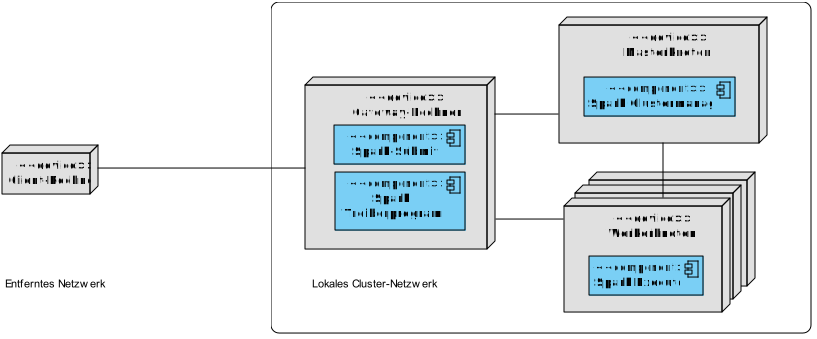
\includegraphics[scale=0.62]{spark_deployment_clientmode.pdf}
	\caption{Application Deployment im Client Modus}
	\label{fig:spark_deployment_clientmode}
\end{figure}\\

\begin{figure}[ht!]
	\centering
  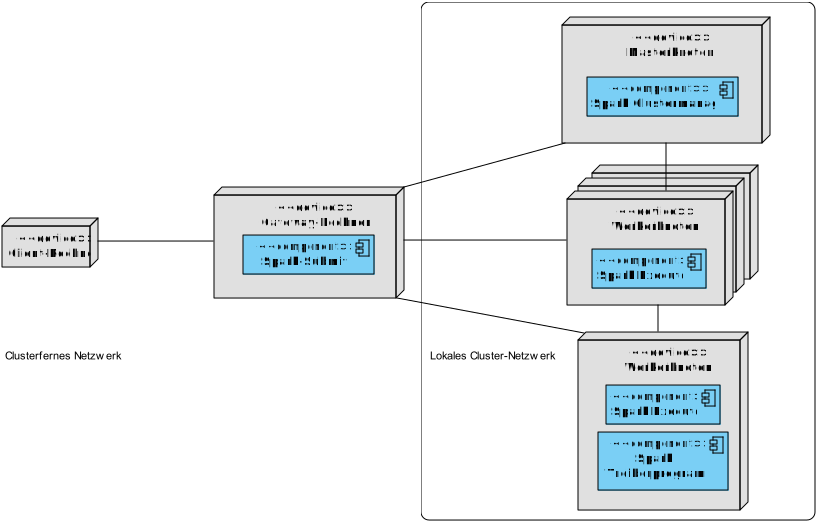
\includegraphics[scale=0.62]{spark_deployment_clustermode.pdf}
	\caption{Application Deployment im Cluster Modus}
	\label{fig:spark_deployment_clustermode}
\end{figure}\\

Offensichtlich kann die Lokalität des Treibers (der mit den Executors auf den \gls{worker}n kommunizieren muss) Einfluss auf Laufzeit und Latenzverhalten des Programms haben.\\

Im Fall eines clusterfernen Gateway-Rechners kann also Treiberdeployment im Clustermodus sinnvoll sein, die Standardeinstellung ist jedoch der Clientmodus (siehe auch \cite{spark_submission}).\\

Abb.~\ref{fig:app_deployment_process} zeigt das Sequenzdiagramm eines typischen Deploymentprozesses, wie er auch im praktischen Teil dieser Arbeit zum Einsatz kommt.

\begin{figure}[ht!]
	\centering
  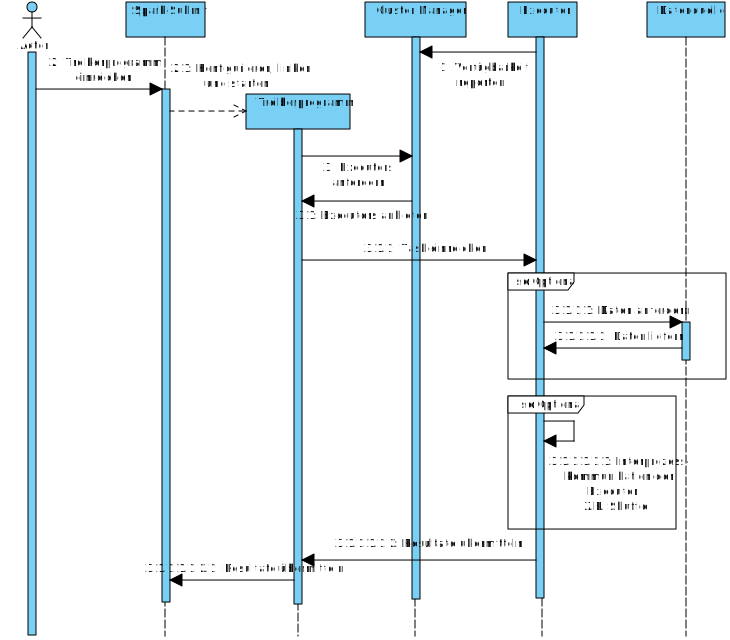
\includegraphics[scale=0.7]{spark_deployment_process.pdf}
	\caption{Application Deployment Prozess im Client Modus (vereinfacht)}
	\label{fig:app_deployment_process}
\end{figure}

\paragraph{Lebenszyklus einer Spark-Applikation}

\textcolor{gray}{Beginn und End eines Treiberprogramms. Beginn un Ende eines Tasks / Executorallokation?}\\

\subsection{Zusammenfassung und Bewertung}

\section{Standardbibliotheken}
Die vier Standardbibliotheken erweitern die Kern-API für bestimmte, häufig genutzte Aufgaben aus Bereichen der Datenanalyse.\\

Die bedienten Bereiche
\begin{itemize}
	\item Deklaratives Abfragen auf strukturierten Datensätzen (\textit{Spark SQL})
	\item Maschinenlernverfahren (\textit{MLlib})
	\item Echtzeitbehandlung von eingehenden Daten (\textit{Streaming})
	\item Operationen auf Graph-Strukturen (\textit{GraphX})
\end{itemize}
werden in diesem Abschnitt erläutert.

\subsection{Dataframes/Spark SQL}


\subsection{MLlib}
\subsection{Streaming}
\subsection{GraphX}

\section{Betrieb und Security}

\section{Spark im Kontext von Parallelisierungspattern}
\textcolor{gray}{--- Buch: Algorithms and Parallel Computing ---}\\

\section{Entwicklergemeinschaft}
\textcolor{gray}{--- Herkunft, Apache Foundation, Entwicklungsphilosophien, Anzahl Entwickler, ... ---}\\

Apache Spark begann als Entwicklung einer Gruppe von Forschern der University of California, Berkely. Spark ist eine Implementation der von dieser Gruppe untersuchten \glspl{rdd}\cite{Mat12}. Als wesentlicher Meilenstein der Entwicklung von Apache Spark, kann die Veröffentlichung eines gemeinsamen Papers der Forschungsgruppe um Matei Zaharia im Jahr 2012 gelten.\\

Seit dem 27. Februar 2014\cite{apacheblog} ist Spark ein Top-Level Projekt der Apache Software Foundation\cite{apache} und wird dort unter der Apache License 2.0\cite{apachelic} weiterentwickelt.\\

Eine Übersicht der verantwortlichen Committer kann unter \cite{committer} eingesehen werden.
Zum Zeitpunkt dieser Arbeit gehören u.a. Entwickler von Intel, Yahoo! und Alibaba zu den Stammentwicklern.\\

Die Kommunikation innerhalb der Entwickler- und Anwendergemeinschaft findet wesentlich in den offiziellen Mailinglisten (Abb. \ref{fig:mailinglisten}) und dem Issue-Tracker\cite{issuetracker} der Apache Software Foundation statt.

\begin{figure}[ht!]
	\centering
	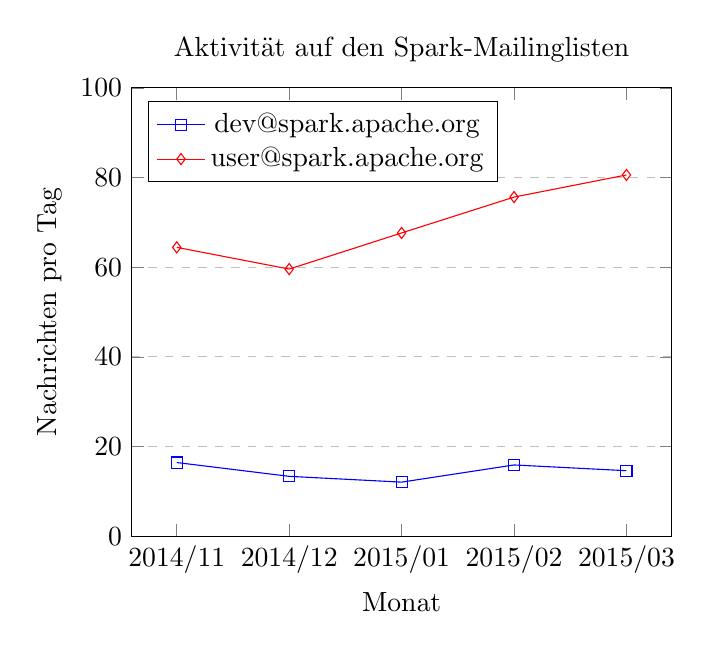
\begin{tikzpicture}
	\begin{axis}[
			title={Aktivität auf den Spark-Mailinglisten},
			xlabel={Monat},
			ylabel={Nachrichten pro Tag},
			%xmin=0, xmax=100,
			ymin=0, ymax=100,
			symbolic x coords={2014/11,2014/12,2015/01,2015/02,2015/03},
			ytick={0,20,40,60,80,100},
			legend pos=north west,
			ymajorgrids=true,
			grid style=dashed,
	]
	 
	\addplot[
			color=blue,
			mark=square,
			]
			coordinates {
			(2014/11,16.43)
			(2014/12,13.35)
			(2015/01,12.06)
			(2015/02,15.89)
			(2015/03,14.61)
			};

	\addplot[
			color=red,
			mark=diamond,
			]
			coordinates {
			(2014/11,64.43)
			(2014/12,59.58)
			(2015/01,67.64)
			(2015/02,75.64)
			(2015/03,80.58)
			};
			\legend{dev@spark.apache.org,user@spark.apache.org}

	 
	\end{axis}
	\end{tikzpicture}
	\caption{Aktivität auf den offiziellen Spark Mailinglisten}
	\label{fig:mailinglisten}
\end{figure}
\\

\section{Auswahl verwandter Produkte}
Um Spark besser im Bereich bestehender Lösungen einzuordnen werden im Folgenden einige Produkte genannt die häufig zusammen mit Spark verwendet oder ähnliche Aufgaben erfüllen.
\paragraph{Hadoop/YARN}\\
Hadoop lässt sich als eine Art Betriebssystem für Cluster zur Datenanalyse beschreiben. Zu den wesentlichen Komponenten zählen ein Dateisystem (HDFS) ein Datenverarbeitungsmodell (MapReduce) und ein Scheduler (YARN).
Alle genannten Komponenten sind für den fehlertoleranten und skalierbaren Betrieb auf verteilten Hardware-Komponenten vorgesehen.\\
Zwar wird mit MapReduce auch eine Komponente zur Verarbeitung/Analyse von verteilt gespeicherten Daten zu Verfügung gestellt, andere Datenverarbeitungsmodelle können jedoch gleichberechtigt und unter Aufsicht des Ressourcenschedulers YARN betrieben werden.\\

Spark liefert eine mögliche Implementation eines solchen alternativen Datenverarbeitungsmodells.

\paragraph{Mesos}\\
Apache Mesos ist seit Beginn der Entwicklung von Spark ein optionaler Clustermanager für Sparkapplikationen \cite{Mat12}.\\
Als reiner Clustermanager ersetzt Mesos die Spark Master-Komponente in der Funktion des knotenübergreifenden Ressourcenmanagements.\\
Wie bei YARN ermöglicht dies auch anderen Anwendungen die über Mesos verwaltet werden einen gleichberechtigten Betrieb auf dem selben Cluster.\\

\paragraph{Flink}\\

\paragraph{MPI}\\

\paragraph{Samza}\\

\paragraph{Storm}\\
